% 'draft' mode can be used to speed up compilation
\documentclass[twoside,final]{hcmut-report}
\usepackage{codespace}
\usepackage{array}

% Draft watermark
% https://github.com/callegar/LaTeX-draftwatermark

% Encodings
\usepackage{gensymb,textcomp}

% Better tables
% Wide tables go to https://tex.stackexchange.com/q/332902
\usepackage{array,longtable,multicol,multirow,siunitx,tabularx}
\usepackage{longtable}

% \setcounter{secnumdepth}{4}
% \setcounter{tocdepth}{4}
% \makeatletter
% \newcounter{subsubsubsection}[subsubsection]
% \renewcommand\thesubsubsubsection{\thesubsubsection .\@arabic\c@subsubsubsection}
% \newcommand\subsubsubsection{\@startsection{subsubsubsection}{4}{\z@}%
%                                      {-3.25ex\@plus -1ex \@minus -.2ex}%
%                                      {1.5ex \@plus .2ex}%
%                                      {\normalfont\normalsize\bfseries}}
% \newcommand*\l@subsubsubsection{\@dottedtocline{4}{10.0em}{4.1em}}
% \makeatother

% Better enum
\usepackage{enumitem}

% Graphics
\usepackage{caption,float}

% Add options for figures, like max width, framing, etc.
\usepackage[export]{adjustbox}

% References
% Use \Cref{} instead of \ref{}
\usepackage[nameinlink]{cleveref}

% FOR DEMONSTRATION PURPOSES, REMOVE IN PRODUCTION
\usepackage{mwe}

% Sub-preambles
% https://github.com/MartinScharrer/standalone

% Configurations
\coursename{Thiết kế vi mạch (CO3097)}
\reporttype{BÀI TẬP LỚN}
\title{Thiết kế RISC CPU}
\advisor{Nguyễn Thành Lộc}
\stuname{%
 & Võ Nguyên Giáp   & 2110142 \\ 
 & Nguyễn Anh Khoa  & 2053134 \\
 & Phan Thanh Bình  & 2110826 \\
 & Hồng Thiện Nhân  & 2111900 \\
 & Bùi Xuân Bách    & 2210179 \\
}
\reportplace{Tp. Hồ Chí Minh}
\uniname{Trường Đại học Bách Khoa}
\upperuniname{Đại học Quốc gia TP.HCM}
\deptname{Khoa Khoa học và Kỹ thuật Máy tính}
\reporttime{Tháng 05 năm 2025}

% Allow page breaks inside align* environment
%\allowdisplaybreaks{}

% Makes a lot of things blue, avoid at all costs
%\everymath{\color{blue}}

% Set depth of numbering for counters
\AtBeginDocument{\counterwithin{lstlisting}{section}}

% Rename some sections
%\AtBeginDocument{\renewcommand*{\contentsname}{Contents}}
%\AtBeginDocument{\renewcommand*{\refname}{References}}
%\AtBeginDocument{\renewcommand*{\bibname}{References}}

% Custom commands
%\newcommand*\mean[1]{\bar{#1}}

\begin{document}
\coverpage

\tableofcontents
\listoffigures
\listoftables
\lstlistoflistings{}

\clearpage
% \section{Normal section}
% This is how you normally work with \LaTeX, but you can also split a project into smaller files for easier management.
% To import other files, you can use \mintinline{latex}{\input{}} or \mintinline{latex}{\include{}}.
% There differences can be found at \url{https://tex.stackexchange.com/a/250}, but in short

% \begin{center}
%   \mintinline{latex}{\include{filename}} = \mintinline{latex}{\clearpage \input{filename} \clearpage}
% \end{center}

% \section{Label prefixes}
% There are no definite rules for label prefixes, but you can use the following as a guideline.
% \begin{itemize}
%   \item \textbf{chap:} for chapters
%   \item \textbf{sec:} for sections
%   \item \textbf{subsec:} for subsections
%   \item \textbf{eq:} for equations
%   \item \textbf{fig:} for figures
%   \item \textbf{tab:} for tables
%   \item \textbf{enum:} for enumerators and items
%   \item \textbf{fn:} for footnotes
%   \item \textbf{lst:} for listings
%   \item \textbf{alg:} for algorithms
%   \item \textbf{app:} for appendices
% \end{itemize}

% The \mintinline{latex}{\caption} macro increases the used counter and sets the current label text which is used by \mintinline{latex}{\label}.
% If you use \mintinline{latex}{\label} before it the old label text is used instead, which leads to a wrong number.
% Always use \mintinline{latex}{\label} after \mintinline{latex}{\caption} and not before or in it.

% That said, conventions are just conventions, and you can use whatever you want as long as you are consistent.

% \clearpage
% \section{Better tables}
The recommended way is by using the \mintinline{latex}{booktabs} package and drop all vertical rules.

\mintinline{latex}{tabularx} is simply tabular but with X environment, meaning that it will try to use all of \mintinline{latex}{\linewidth}.

\begin{table}[H]
  \centering
  \caption{Tabularx table}%
  \label{tab:tabularx}
  \begin{tabularx}{\linewidth}{l*{2}{X}}
    \toprule
         & OOP & FP \\
    \cmidrule(lr){2-3}
    Pros &     &    \\
         &     &    \\
         &     &    \\
    \midrule
    Cons &     &    \\
         &     &    \\
         &     &    \\
    \bottomrule
  \end{tabularx}
\end{table}

More information can be found at \url{https://latex-tutorial.com/tables-in-latex/}.

In \mintinline{latex}{tabular}, with the \mintinline{latex}{p}, \mintinline{latex}{m} or \mintinline{latex}{b} column types, sometimes you will notice that the width of the table is wider than the sum of the widths of the columns.
This is due to the padding added by the \mintinline{latex}{\tabcolsep} and the line width of the vertical separators which are added by default.

\begin{code}{latex}
  \tabcolsep + p{length} + \tabcolsep
\end{code}

By default, \mintinline{latex}{tabcolsep} is set to 6pt, which equals to 2.12mm in digital printing.
The use of \mintinline{latex}{@{}..@{}} voids this behavior.

Additionally, if you have to insert a very long table, which takes up two or more pages in your document, use the \mintinline{latex}{longtable} package.

\begin{longtable}[H]{|m{0.3\linewidth}|m{0.3\linewidth}|}
  \caption{Long table caption}\label{tab:long}          \\
  \toprule
  \multicolumn{2}{|c|}{Begin of Table}                  \\
  \midrule
  Something     & something else                        \\
  \midrule
  \endfirsthead

  \toprule
  \multicolumn{2}{|c|}{Continuation of \Cref{tab:long}} \\
  \midrule
  Something     & something else                        \\
  \midrule
  \endhead

  \midrule
  \endfoot

  \midrule
  \multicolumn{2}{|c|}{End of Table}                    \\
  \bottomrule
  \endlastfoot

  Lots of lines & like this                             \\
  Lots of lines & like this                             \\
  Lots of lines & like this                             \\
  Lots of lines & like this                             \\
  Lots of lines & like this                             \\
  Lots of lines & like this                             \\
  Lots of lines & like this                             \\
  Lots of lines & like this                             \\
  Lots of lines & like this                             \\
  Lots of lines & like this                             \\
  Lots of lines & like this                             \\
  Lots of lines & like this                             \\
  Lots of lines & like this                             \\
  Lots of lines & like this                             \\
  Lots of lines & like this                             \\
  Lots of lines & like this                             \\
  Lots of lines & like this                             \\
  Lots of lines & like this                             \\
  Lots of lines & like this                             \\
  Lots of lines & like this                             \\
  Lots of lines & like this                             \\
  Lots of lines & like this                             \\
  Lots of lines & like this                             \\
  Lots of lines & like this                             \\
  Lots of lines & like this                             \\
  Lots of lines & like this                             \\
  Lots of lines & like this                             \\
  Lots of lines & like this                             \\
  Lots of lines & like this                             \\
  Lots of lines & like this                             \\
  Lots of lines & like this                             \\
  Lots of lines & like this                             \\
  Lots of lines & like this                             \\
  Lots of lines & like this                             \\
  Lots of lines & like this                             \\
  Lots of lines & like this                             \\
  Lots of lines & like this                             \\
  Lots of lines & like this                             \\
  Lots of lines & like this                             \\
  Lots of lines & like this                             \\
  Lots of lines & like this                             \\
  Lots of lines & like this                             \\
  Lots of lines & like this                             \\
  Lots of lines & like this                             \\
  Lots of lines & like this                             \\
  Lots of lines & like this                             \\
  Lots of lines & like this                             \\
  Lots of lines & like this                             \\
  Lots of lines & like this                             \\
  Lots of lines & like this                             \\
  Lots of lines & like this                             \\
  Lots of lines & like this                             \\
  Lots of lines & like this                             \\
  Lots of lines & like this                             \\
  Lots of lines & like this                             \\
  Lots of lines & like this                             \\
  Lots of lines & like this                             \\
  Lots of lines & like this                             \\
  Lots of lines & like this                             \\
  Lots of lines & like this                             \\
  Lots of lines & like this                             \\
  Lots of lines & like this                             \\
  Lots of lines & like this                             \\
\end{longtable}

You may use the \mintinline{latex}{\label} command so that you can cross reference longtables with \mintinline{latex}{\ref}.
Note however, that the \mintinline{latex}{\label} command should not be used in a heading that may appear more than once.
Place it either in the firsthead, or in the body of the table.
It should not be the first command in any entry.

% \section{Better enumerator}
Normal enumerator gets the job done, but what if you want custom numbering?
This implementation allows custom labeling, either by pre-defined rules or in-place.

\begin{enumerate}[start=4,label={\alph*.yeah}]
  \item First item
  \item Second item
  \item[custom] Third item
\end{enumerate}

% \section{Codespace}
\subsection{Listings}
This is the recommended way to insert simple code.

\begin{itemize}
  \item \lstinputlisting[
    language=python,
    caption={External import},name=ext-import,label=lst:ext-import
  ]{code/example.py}

  \item \lstinputlisting[
    firstline=10,lastline=13,language=python,
    caption={External import but with a line range},
    name=line-range,label=lst:line-range
  ]{code/example.py}

  \item \begin{lstlisting}[
    language=python,caption={Embedded},name=embedded,label=lst:embedded
  ]
  from typing import Iterator

  # This is an example
  class Math:
      @staticmethod
      def fib(n: int) -> Iterator[int]:
          """Fibonacci series up to n."""
          a, b = 0, 1
          while a < n:
              yield a
              a, b = b, a + b

  result = sum(Math.fib(42))
  print("The answer is {}".format(result))
  \end{lstlisting}

  \item Inline

  \lstinline[
    language=python,
    name=inline,label=lst:inline
  ]{print('Hello, world!')}
\end{itemize}

\subsection{Minted}
This provide better looking code, but requires external setup:

\emph{Minted requires python Pygments and the \mintinline{text}{--shell-escape} flag.}

\begin{itemize}
  \item External import

  \inputcode[highlightlines={1,10-13}]{Python}{code/example.py}

  \item With a line range

  \inputcode[firstnumber=1,firstline=10,lastline=13]{Python}{code/example.py}

  \item Embedded

  \begin{code}{python}
  from typing import Iterator

  # This is an example
  class Math:
      @staticmethod
      def fib(n: int) -> Iterator[int]:
          """Fibonacci series up to n."""
          a, b = 0, 1
          while a < n:
              yield a
              a, b = b, a + b

  result = sum(Math.fib(42))
  print("The answer is {}".format(result))
  \end{code}

  \item Inline

  \mintinline{Python}{print('Hello, world!')}
\end{itemize}

% \section{Figures with flexible width}

\hrule % to see \linewidth

\begin{figure}[H]
  \includegraphics[max width=0.9\linewidth]{example-image-1x1}
  \caption{Example image 1x1}%
  \label{fig:example-image-1x1}
\end{figure}

\begin{figure}[H]
  \includegraphics[frame,scale=0.7]{example-image-a4}
  \caption{Example image A4}%
  \label{fig:example-image-a4}
\end{figure}

With \mintinline{latex}{\adjincludegraphics} (or \mintinline{latex}{\adjustimage}) you can also use the original width as \mintinline{latex}{\width}:

\begin{figure}[H]
  \adjincludegraphics[width=\ifdim \width > \linewidth \linewidth \else \width \fi]{example-image}
  \caption{Set figure width imperatively}%
  \label{fig:imperative-width}
\end{figure}


\chapter{Interface}
\chapter{Functional Implementation}
\section{Tổng quan kiến trúc tập lệnh RISC}
Bộ xử lý RISC (Reduced Instruction Set Computer) được thiết kế với tập lệnh đơn giản và hiệu quả nhằm tối ưu hóa quá trình thực thi chương trình. Trong thiết kế này, chúng tôi phát triển một RISC CPU đơn giản với các thông số cơ bản:

\begin{itemize}
    \item Kiến trúc lệnh 8-bit với cấu trúc: 3-bit opcode + 5-bit toán hạng

    \item Không gian địa chỉ 32 vị trí ($2^{5} = 32$ địa chỉ)

    \item Bộ nhớ dữ liệu 8-bit
    
    \item Thanh ghi tích lũy (Accumulator) 8-bit
    \item Bộ đếm chương trình (Program Counter) 5-bit
   
\end{itemize}

Dựa trên sơ đồ khối tổng quát (Hình ở chương 3), RISC CPU được thiết kế với các khối chức năng chính sau:

\begin{enumerate}

    \item \textbf{Program Counter (PC): }Lưu trữ địa chỉ của lệnh tiếp theo được thực thi
    \item \textbf{Address Multiplexer (Mux): }Lựa chọn giữa địa chỉ lệnh và địa chỉ dữ liệu
    \item \textbf{Memory: } Lưu trữ cả lệnh và dữ liệu

    \item \textbf{Instruction Register (IR): }Lưu trữ lệnh hiện tại đang được thực thi
    \item \textbf{Controller: }Điều khiển hoạt động của toàn bộ hệ thống
    \item \textbf{Accumulator Register (AC): }Lưu trữ dữ liệu và kết quả tính toán
    \item \textbf{Arithmetic Logic Unit (ALU): }Thực hiện các phép toán số học và logic
\end{enumerate}

\subsection{Cấu trúc lệnh}

Định dạng lệnh của CPU được thiết kế đơn giản với 8-bit, trong đó:
\begin{itemize}
    \item 3 bit cao nhất (bit 7-5) biểu diễn mã lệnh (opcode)
    \item 5 bit thấp nhất (bit 4-0) biểu diễn địa chỉ toán hạng hoặc giá trị trực tiếp (immediate value)
\end{itemize}

\begin{figure}[h]
\centering
\begin{tabular}{|c|c|}
\hline
Opcode[3] & Operand[5] \\
\hline
Bit 7-5 & Bit 4-0 \\
\hline
\end{tabular}
\caption{Cấu trúc lệnh 8-bit của RISC CPU}
\label{fig:instruction_format}
\end{figure}

Cấu trúc này cho phép CPU hỗ trợ tối đa 8 lệnh khác nhau ($2^3 = 8$) và có thể truy cập đến 32 ô nhớ dữ liệu khác nhau ($2^5 = 32$).

\subsection{Bộ lệnh}

RISC CPU hỗ trợ 8 lệnh cơ bản (mỗi lệnh tương ứng với một opcode):

\begin{table}[h]
\centering
\begin{tabular}{|c|c|l|p{0.5\textwidth}|}
\hline
\textbf{Opcode} & \textbf{Mnemonic} & \textbf{Chức năng} & \textbf{Hoạt động} \\
\hline
000 & HLT & Halt & Dừng hoạt động chương trình \\
\hline
001 & SKZ & Skip if Zero & Kiểm tra ALU, nếu kết quả = 0 thì bỏ qua lệnh tiếp theo \\
\hline
010 & ADD & Add & Accumulator = Accumulator + Memory[address] \\
\hline
011 & AND & Logical AND & Accumulator = Accumulator AND Memory[address] \\
\hline
100 & XOR & Logical XOR & Accumulator = Accumulator XOR Memory[address] \\
\hline
101 & LDA & Load Accumulator & Accumulator = Memory[address] \\
\hline
110 & STO & Store Accumulator & Memory[address] = Accumulator \\
\hline
111 & JMP & Jump & Program Counter = address \\
\hline
\end{tabular}
\caption{Bộ lệnh của RISC CPU}
\label{tab:instruction_set}
\end{table}

\section{Hoạt động chức năng của CPU}

\subsection{Luồng dữ liệu}

Dựa trên sơ đồ khối, luồng dữ liệu trong RISC CPU được phân thành ba đường chính:

\begin{enumerate}
    \item \textbf{Đường Address Bus} (màu xanh lá trong sơ đồ)
    \begin{itemize}
        \item Xuất phát từ Program Counter hoặc phần toán hạng của Instruction Register
        \item Đi qua Address Mux để lựa chọn nguồn địa chỉ
        \item Kết nối đến Memory để truy xuất dữ liệu hoặc lệnh
    \end{itemize}

    \item \textbf{Đường Data Bus} (màu xanh dương trong sơ đồ)
    \begin{itemize}
        \item Kết nối dữ liệu giữa Memory, Instruction Register, Accumulator và ALU
        \item Truyền dữ liệu hai chiều giữa Memory và các thành phần xử lý
        \item Dùng để lấy lệnh từ bộ nhớ và nạp vào IR
        \item Dùng để truyền dữ liệu giữa Memory và Accumulator
    \end{itemize}
    
    \item \textbf{Đường Control Lines} (màu đỏ trong sơ đồ)
    \begin{itemize}
        \item Điều khiển từ Controller đến tất cả các module khác
        \item Bao gồm các tín hiệu: sel, rd, ld\_ir, halt, inc\_pc, ld\_ac, ld\_pc, wr, data\_e
        \item Định hướng hoạt động trong từng chu kỳ xử lý
    \end{itemize}
\end{enumerate}

\subsection{Chu trình thực thi lệnh}

RISC CPU hoạt động theo chu trình lấy lệnh và thực thi (Fetch-Execute cycle) được phân chia thành 8 trạng thái tuần tự:

\begin{enumerate}
    \item \textbf{INST\_ADDR}: Cài đặt địa chỉ cho việc lấy lệnh
    \begin{itemize}
        \item PC chứa địa chỉ lệnh cần thực thi
        \item Controller đặt sel=1 để Address Mux chọn địa chỉ từ PC
    \end{itemize}
    
    \item \textbf{INST\_FETCH}: Lấy lệnh từ bộ nhớ
    \begin{itemize}
        \item Controller đặt rd=1 để đọc dữ liệu từ Memory
        \item Dữ liệu từ Memory được đưa lên Data Bus
    \end{itemize}

    \item \textbf{INST\_LOAD}: Nạp lệnh vào thanh ghi lệnh (IR)
    \begin{itemize}
        \item Controller đặt ld\_ir=1 để nạp dữ liệu từ Data Bus vào IR
        \item IR phân tách thành opcode và địa chỉ toán hạng
    \end{itemize}

    \item \textbf{IDLE}: Trạng thái nghỉ/chờ
    \begin{itemize}
        \item CPU xử lý opcode để quyết định hành động tiếp theo
        \item Controller kiểm tra nếu opcode là HLT để dừng chương trình
    \end{itemize}

    \item \textbf{OP\_ADDR}: Cài đặt địa chỉ cho việc lấy toán hạng
    \begin{itemize}
        \item Controller đặt sel=0 để Address Mux chọn địa chỉ từ toán hạng của IR
        \item Địa chỉ được đưa đến Memory
    \end{itemize}

    \item \textbf{OP\_FETCH}: Lấy toán hạng từ bộ nhớ
    \begin{itemize}
        \item Controller đặt rd=1 (đối với các lệnh ADD, AND, XOR, LDA)
        \item Dữ liệu từ Memory được đưa đến ALU qua đường inB
    \end{itemize}

    \item \textbf{ALU\_OP}: Thực hiện phép toán trên ALU
    \begin{itemize}
        \item ALU thực hiện phép toán dựa trên opcode
        \item Dữ liệu từ Accumulator được đưa vào inA của ALU
        \item Kết quả được chuẩn bị để nạp vào Accumulator
    \end{itemize}

    \item \textbf{STORE}: Lưu kết quả vào bộ nhớ hoặc thanh ghi
    \begin{itemize}
        \item Đối với lệnh STO: Controller đặt wr=1, data\_e=1 để ghi dữ liệu từ Accumulator vào Memory
        \item Đối với các lệnh khác: Controller đặt ld\_ac=1 để nạp kết quả từ ALU vào Accumulator
    \end{itemize}
\end{enumerate}

Chu trình này được lặp lại liên tục cho đến khi gặp lệnh HLT hoặc có tín hiệu reset.

\subsection{Cơ chế thực thi từng lệnh}

\subsubsection{HLT (Halt - 000)}
\begin{itemize}
    \item \textbf{Mô tả}: Dừng hoạt động của CPU
    \item \textbf{Thực thi}: 
    \begin{itemize}
        \item Khi nhận opcode HLT, tín hiệu halt được kích hoạt
        \item CPU dừng thực hiện các chu kỳ lệnh tiếp theo
    \end{itemize}
    \item \textbf{Ứng dụng}: Kết thúc chương trình
\end{itemize}

\subsubsection{SKZ (Skip if Zero - 001)}
\begin{itemize}
    \item \textbf{Mô tả}: Kiểm tra kết quả trong Accumulator, nếu bằng 0 thì bỏ qua lệnh tiếp theo
    \item \textbf{Thực thi}:
    \begin{itemize}
        \item ALU kiểm tra giá trị của Accumulator thông qua tín hiệu is\_zero
        \item Nếu is\_zero = 1 (Accumulator = 0), PC được tăng thêm 1 lần nữa
    \end{itemize}
    \item \textbf{Ứng dụng}: Điều kiện rẽ nhánh cho cấu trúc điều khiển
\end{itemize}

\subsubsection{ADD (Add - 010)}
\begin{itemize}
    \item \textbf{Mô tả}: Cộng giá trị từ bộ nhớ vào Accumulator
    \item \textbf{Thực thi}:
    \begin{itemize}
        \item Lấy giá trị tại địa chỉ operand từ bộ nhớ
        \item ALU thực hiện phép cộng: Accumulator + Memory[address]
        \item Kết quả được nạp lại vào Accumulator
    \end{itemize}
    \item \textbf{Ứng dụng}: Thực hiện phép tính cộng trong các ứng dụng số học
\end{itemize}

\subsubsection{AND (Logical AND - 011)}
\begin{itemize}
    \item \textbf{Mô tả}: Thực hiện phép AND logic giữa Accumulator và giá trị từ bộ nhớ
    \item \textbf{Thực thi}:
    \begin{itemize}
        \item Lấy giá trị tại địa chỉ operand từ bộ nhớ
        \item ALU thực hiện phép AND bit: Accumulator \& Memory[address]
        \item Kết quả được nạp lại vào Accumulator
    \end{itemize}
    \item \textbf{Ứng dụng}: Thao tác bit, kiểm tra bit mask
\end{itemize}

\subsubsection{XOR (Logical XOR - 100)}
\begin{itemize}
    \item \textbf{Mô tả}: Thực hiện phép XOR logic giữa Accumulator và giá trị từ bộ nhớ
    \item \textbf{Thực thi}:
    \begin{itemize}
        \item Lấy giá trị tại địa chỉ operand từ bộ nhớ
        \item ALU thực hiện phép XOR bit: Accumulator $\oplus$ Memory[address]
        \item Kết quả được nạp lại vào Accumulator
    \end{itemize}
    \item \textbf{Ứng dụng}: Thao tác bit, mã hóa/giải mã đơn giản
\end{itemize}

\subsubsection{LDA (Load Accumulator - 101)}
\begin{itemize}
    \item \textbf{Mô tả}: Nạp giá trị từ bộ nhớ vào Accumulator
    \item \textbf{Thực thi}:
    \begin{itemize}
        \item Lấy giá trị tại địa chỉ operand từ bộ nhớ
        \item Giá trị này được nạp trực tiếp vào Accumulator
    \end{itemize}
    \item \textbf{Ứng dụng}: Khởi tạo giá trị, đọc dữ liệu
\end{itemize}

\subsubsection{STO (Store Accumulator - 110)}
\begin{itemize}
    \item \textbf{Mô tả}: Lưu giá trị từ Accumulator vào bộ nhớ
    \item \textbf{Thực thi}:
    \begin{itemize}
        \item Giá trị từ Accumulator được ghi vào bộ nhớ tại địa chỉ operand
    \end{itemize}
    \item \textbf{Ứng dụng}: Lưu kết quả tính toán, ghi dữ liệu
\end{itemize}

\subsubsection{JMP (Jump - 111)}
\begin{itemize}
    \item \textbf{Mô tả}: Nhảy đến địa chỉ được chỉ định để thực thi
    \item \textbf{Thực thi}:
    \begin{itemize}
        \item Giá trị operand được nạp trực tiếp vào Program Counter
        \item Lệnh tiếp theo sẽ được lấy từ địa chỉ mới
    \end{itemize}
    \item \textbf{Ứng dụng}: Vòng lặp, rẽ nhánh không điều kiện
\end{itemize}

\section{Các cơ chế đặc biệt}

\subsection{Xử lý điều kiện rẽ nhánh}

CPU được thiết kế với khả năng rẽ nhánh có điều kiện thông qua phối hợp SKZ và JMP:

\begin{itemize}
    \item \textbf{Rẽ nhánh có điều kiện}: Sử dụng SKZ để kiểm tra điều kiện (Accumulator = 0), nếu thỏa mãn thì bỏ qua lệnh JMP kế tiếp.
    \item \textbf{Rẽ nhánh không điều kiện}: Sử dụng JMP để nhảy trực tiếp đến địa chỉ đích.
\end{itemize}

Ví dụ mẫu lệnh rẽ nhánh có điều kiện:
\begin{verbatim}
LDA A    ; Nạp giá trị A vào Accumulator
SKZ      ; Kiểm tra nếu A = 0
JMP ELSE ; Nếu A != 0, nhảy đến nhãn ELSE
; Đoạn code khi A = 0
JMP END  ; Nhảy đến kết thúc
ELSE:    ; Nhãn ELSE
; Đoạn code khi A != 0
END:     ; Nhãn kết thúc
\end{verbatim}

\subsection{Tạo vòng lặp}

CPU có thể thực hiện vòng lặp thông qua phối hợp các lệnh tính toán, so sánh và nhảy:

Ví dụ vòng lặp đếm từ 5 về 0:
\begin{verbatim}
LDA COUNT  ; Nạp giá trị ban đầu (5)
LOOP:
STO COUNT  ; Lưu giá trị hiện tại
LDA ONE    ; Nạp giá trị 1
SKZ        ; Kiểm tra nếu giá trị = 0 (không xảy ra)
ADD NEG_ONE; Giảm bộ đếm (Accumulator = Accumulator - 1)
SKZ        ; Kiểm tra nếu đã đếm về 0
JMP LOOP   ; Nếu chưa về 0, lặp lại
; Tiếp tục chương trình khi vòng lặp kết thúc
\end{verbatim}

\section{ABC - Chi tiết thiết kế bộ điều khiển}

Bộ điều khiển (Controller) là thành phần trung tâm điều phối tất cả hoạt động của CPU. Trong thiết kế này, bộ điều khiển được hiện thực dưới dạng máy trạng thái hữu hạn (Finite State Machine - FSM).

\subsection{Tín hiệu điều khiển}

Các tín hiệu đầu ra từ Controller điều khiển hoạt động của toàn bộ hệ thống:

\begin{table}[h]
\centering
\begin{tabular}{|l|l|}
\hline
\textbf{Tín hiệu} & \textbf{Chức năng} \\
\hline
sel & Lựa chọn giữa địa chỉ từ PC (sel=1) hoặc địa chỉ toán hạng (sel=0) \\
\hline
rd & Kích hoạt chế độ đọc dữ liệu từ Memory \\
\hline
ld\_ir & Nạp dữ liệu vào Instruction Register \\
\hline
halt & Dừng hoạt động của CPU \\
\hline
inc\_pc & Tăng Program Counter lên 1 \\
\hline
ld\_ac & Nạp dữ liệu vào Accumulator \\
\hline
ld\_pc & Nạp địa chỉ mới vào Program Counter \\
\hline
wr & Kích hoạt chế độ ghi dữ liệu vào Memory \\
\hline
data\_e & Cho phép đưa dữ liệu từ Accumulator lên Data Bus \\
\hline
\end{tabular}
\caption{Các tín hiệu điều khiển của Controller}
\label{tab:control_signals}
\end{table}

\subsection{Máy trạng thái cho chu trình lệnh}

Bộ điều khiển triển khai máy trạng thái 8 trạng thái cho chu trình lệnh. Các tín hiệu điều khiển được tạo ra dựa trên trạng thái hiện tại và opcode của lệnh đang thực thi:

\begin{table}[h]
\centering
\resizebox{\textwidth}{!}{
\begin{tabular}{|l|c|c|c|c|c|c|c|c|c|l|}
\hline
\textbf{Trạng thái} & \textbf{sel} & \textbf{rd} & \textbf{ld\_ir} & \textbf{halt} & \textbf{inc\_pc} & \textbf{ld\_ac} & \textbf{ld\_pc} & \textbf{wr} & \textbf{data\_e} & \textbf{Chú thích} \\
\hline
INST\_ADDR & 1 & 0 & 0 & 0 & 0 & 0 & 0 & 0 & 0 & Đặt địa chỉ lệnh \\
\hline
INST\_FETCH & 1 & 1 & 0 & 0 & 0 & 0 & 0 & 0 & 0 & Đọc lệnh từ bộ nhớ \\
\hline
INST\_LOAD & 1 & 1 & 1 & 0 & 0 & 0 & 0 & 0 & 0 & Nạp lệnh vào IR \\
\hline
IDLE & 1 & 1 & 1 & HALT & 0 & 0 & 0 & 0 & 0 & Giải mã lệnh \\
\hline
OP\_ADDR & 0 & 0 & 0 & 0 & SKZ\&zero & 0 & 0 & 0 & 0 & Đặt địa chỉ toán hạng \\
\hline
OP\_FETCH & 0 & ALUOP & 0 & 0 & 0 & 0 & 0 & 0 & 0 & Đọc toán hạng \\
\hline
ALU\_OP & 0 & ALUOP & 0 & 0 & 0 & 0 & JMP & 0 & 0 & Thực hiện phép toán \\
\hline
STORE & 0 & ALUOP & 0 & 0 & 0 & ALUOP & JMP & STO & STO & Lưu kết quả \\
\hline
\end{tabular}
}
\caption{Máy trạng thái của Controller}
\label{tab:state_machine}
\end{table}

Trong đó:
\begin{itemize}
    \item HALT = 1 khi opcode = 000 (HLT)
    \item SKZ = 1 khi opcode = 001 (SKZ)
    \item ALUOP = 1 khi opcode = 010 (ADD), 011 (AND), 100 (XOR), hoặc 101 (LDA)
    \item STO = 1 khi opcode = 110 (STO)
    \item JMP = 1 khi opcode = 111 (JMP)
    \item zero = tín hiệu is\_zero từ ALU
\end{itemize}

\subsection{Hiện thực tối ưu và mở rộng}

\subsubsection{Tối ưu quá trình thực thi}

Để tối ưu quá trình thực thi, CPU có những điều chỉnh đặc biệt cho các lệnh khác nhau:

\begin{itemize}
    \item \textbf{Xử lý lệnh JMP}: Bộ điều khiển nạp trực tiếp địa chỉ từ toán hạng vào PC trong trạng thái ALU\_OP và STORE, giúp rút ngắn chu kỳ xử lý
    \item \textbf{Xử lý lệnh SKZ}: Tăng PC thêm 1 trong trạng thái OP\_ADDR nếu Accumulator = 0 để bỏ qua lệnh tiếp theo
    \item \textbf{Cơ chế pipeline đơn giản}: Sử dụng IDLE state để giải mã lệnh trong khi chuẩn bị địa chỉ toán hạng
\end{itemize}

\subsubsection{Hướng mở rộng}

CPU có thể được mở rộng trong tương lai theo các hướng:

\begin{itemize}
    \item Bổ sung thêm các lệnh tính toán số học nâng cao như nhân, chia
    \item Mở rộng không gian địa chỉ lên 6-bit hoặc 8-bit
    \item Thêm các thanh ghi đa năng để lưu trữ dữ liệu tạm thời
    \item Hiện thực pipeline nhiều tầng để tăng hiệu suất xử lý
\end{itemize}
\chapter{Internal Implementation}
    \section{Overall}
        \begin{figure}[h]
            \centering
            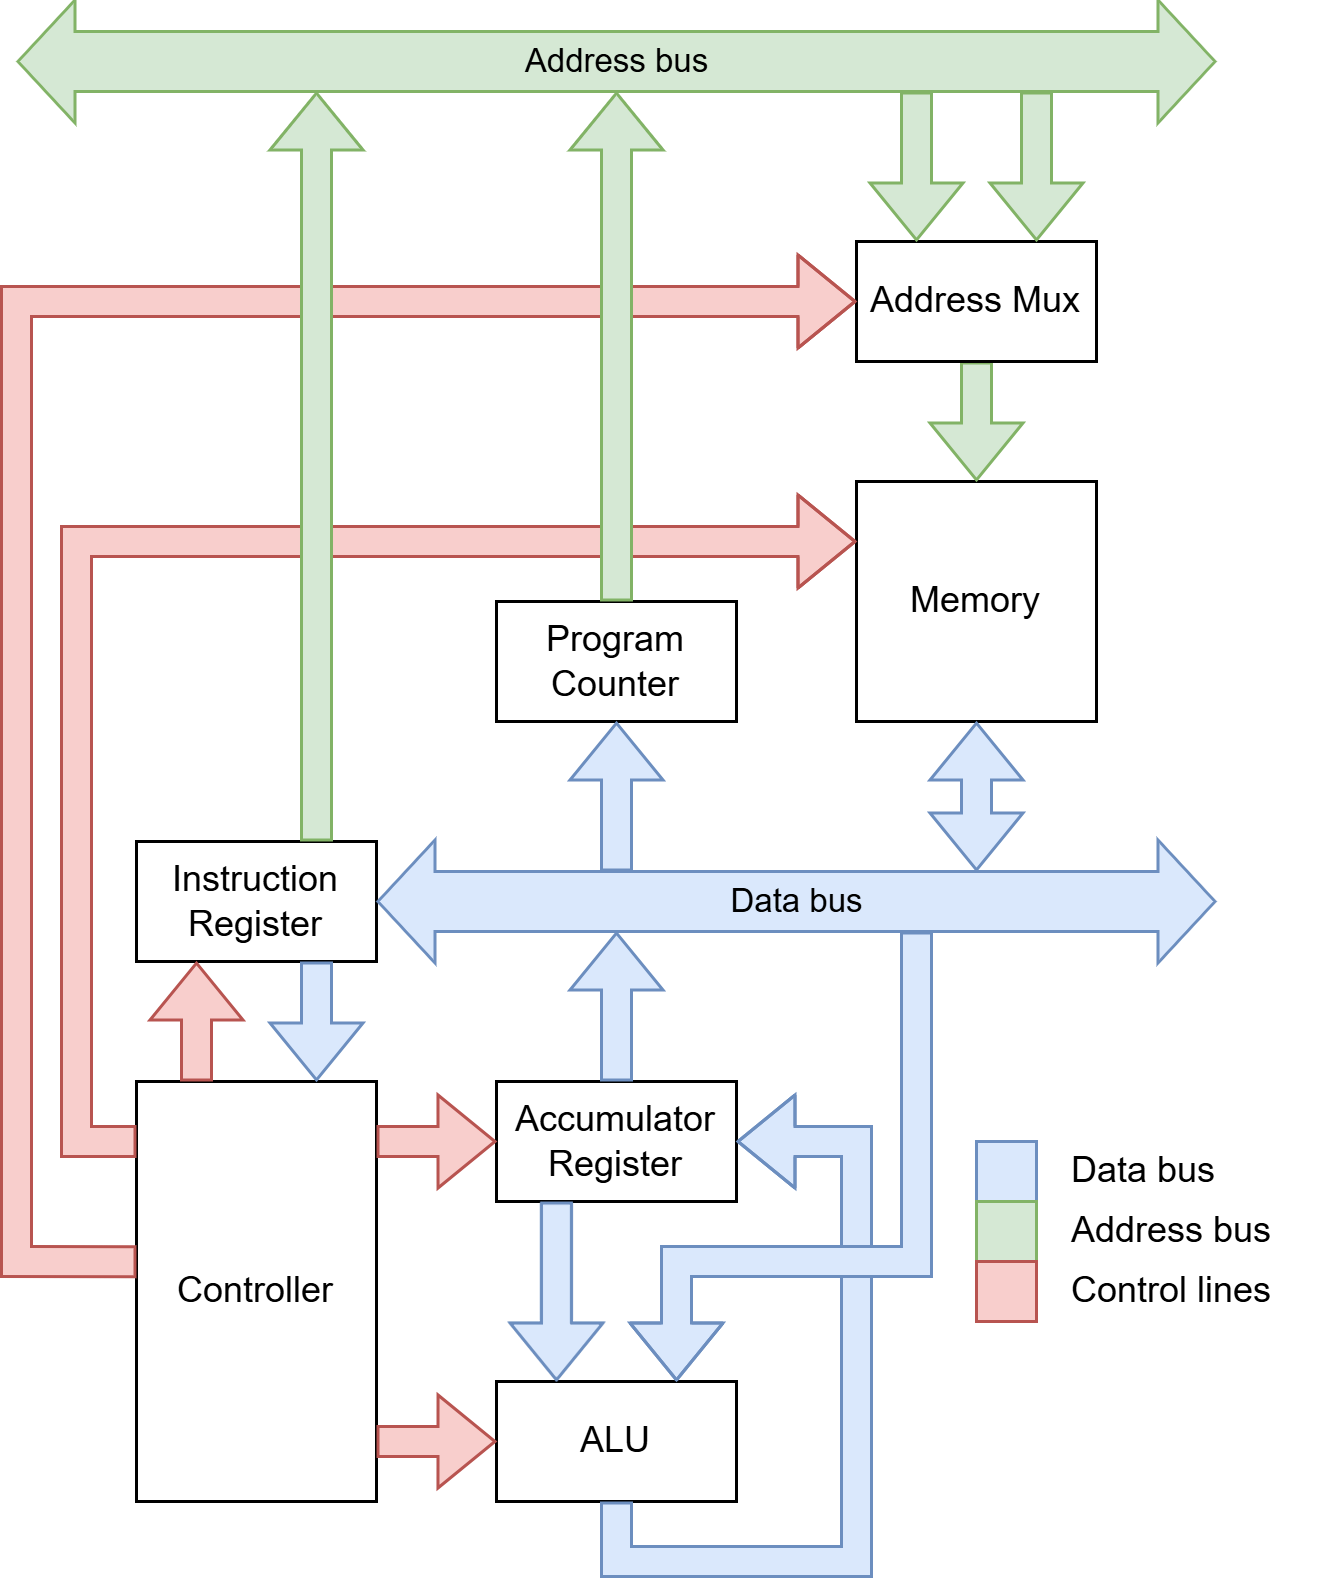
\includegraphics[width=0.6\textwidth]{graphics/RISC-CPU_simple.drawio.png}
            \caption{Sơ đối khối tổng quát của RISC-CPU}
        \end{figure}
        \newpage
        \begin{figure}[h]
            \centering
            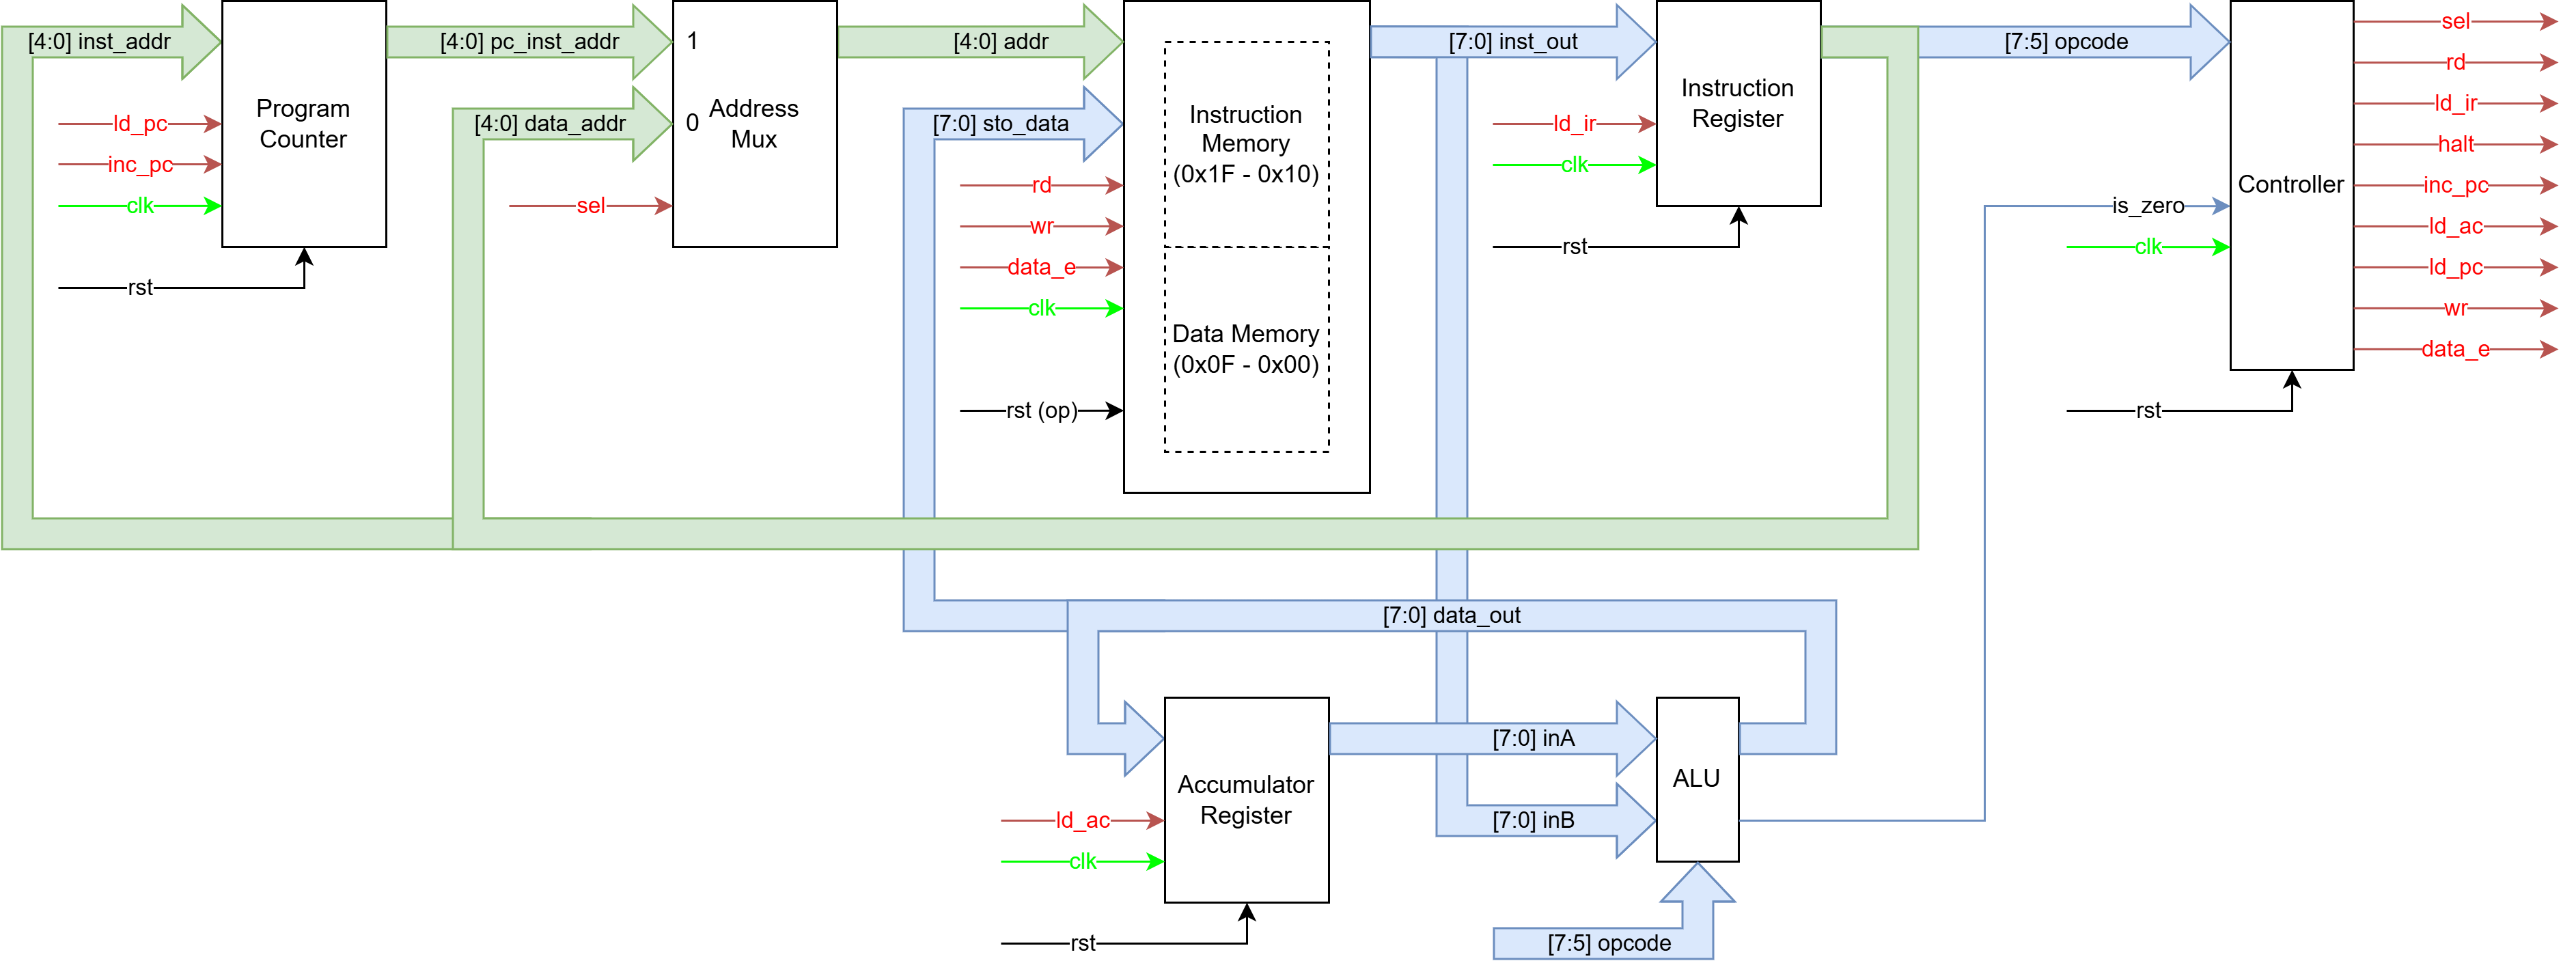
\includegraphics[width=0.8\textwidth]{graphics/RISC-CPU.drawio.png}
            \caption{Sơ đồ khối của RISC-CPU}
        \end{figure}


        \begin{longtable}{|p{0.2\textwidth}|p{0.15\textwidth}|p{0.15\textwidth}|p{0.4\textwidth}|}
            \hline
            \textbf{Tên tín hiệu} & \textbf{Khối phát} & \textbf{Khối nhận} & \textbf{Chức năng} \\
            \hline
            \endfirsthead
            
            \hline
            \textbf{Tên tín hiệu} & \textbf{Khối phát} & \textbf{Khối nhận} & \textbf{Chức năng} \\
            \hline
            \endhead
            
            \hline
            \endfoot
            
            \hline
            \caption{Mô tả tín hiệu của RISC-CPU}
            \endlastfoot
            
            \multicolumn{4}{|c|}{\textbf{Data bus}} \\\hline
            \texttt{inst\_out} & Instruction Memory & Instruction Register & Bus dữ liệu 8-bit tập lệnh. \\
            \hline
            \texttt{opcode} & Instruction Register & Controller, ALU & 3-bit opcode xác định loại lệnh đang thực hiện. \\
            \hline
            \texttt{inA} & Accumulator Register & ALU & Bus dữ liệu 8-bit đầu vào A cho ALU từ Accumulator Register. \\
            \hline
            \texttt{inB} & Data Memory & ALU & Bus dữ liệu 8-bit đầu vào B cho ALU từ Data Memory. \\
            \hline
            \texttt{data\_out} & ALU & Accumulator Register / Data Memory & Bus dữ liệu 8-bit kết quả phép toán từ ALU. \\
            \hline
            \texttt{sto\_data} & ALU & Data Memory & Bus dữ liệu 8-bit ghi vào Data Memory từ Accumulator Register. \\
            \hline
            \texttt{is\_zero} & ALU & Controller & Tín hiệu cho biết kết quả phép toán có bằng 0 hay không (dùng trong lệnh SKZ). \\
            \hline

            \multicolumn{4}{|c|}{\textbf{Address bus}} \\\hline
            \texttt{inst\_addr} & Instruction Register & Program Counter & Bus địa chỉ 5-bit dùng trong lệnh JMP. \\
            \hline
            \texttt{pc\_inst\_addr} & Program Counter & Address Mux & Bus địa chỉ 5-bit từ bộ đếm chương trình. \\
            \hline
            \texttt{data\_addr} & Instruction Register & Address Mux & Bus địa chỉ 5-bit để truy xuất dữ liệu từ Data Memory. \\
            \hline
            \texttt{addr} & Address Mux & Memory & Bus địa chỉ 5-bit được chọn để thực thi lệnh hoặc truy xuất dữ liệu từ Memory. \\
            \hline
            
            \multicolumn{4}{|c|}{\textbf{Control lines}} \\\hline
            \texttt{sel} & Controller & Address Mux & Chọn nguồn địa chỉ: địa chỉ lệnh hoặc địa chỉ dữ liệu. \\
            \hline
            \texttt{rd} & Controller & Memory & Kích hoạt chế độ đọc từ bộ nhớ. \\
            \hline
            \texttt{ld\_ir} & Controller & Instruction Register & Cho phép nạp dữ liệu mới vào Instruction Register. \\
            \hline
            \texttt{halt} & Controller & CPU System & Dừng hoạt động của CPU. \\
            \hline
            \texttt{inc\_pc} & Controller & Program Counter & Tăng địa chỉ Program Counter để nạp lệnh kế tiếp. \\
            \hline
            \texttt{ld\_ac} & Controller & Accumulator Register & Cho phép nạp dữ liệu mới vào Accumulator Register. \\
            \hline
            \texttt{ld\_pc} & Controller & Program Counter & Cho phép nạp địa chỉ mới vào Program Counter (dùng trong lệnh JMP). \\
            \hline
            \texttt{wr} & Controller & Memory & Kích hoạt chế độ ghi xuống bộ nhớ. \\
            \hline
            \texttt{data\_e} & Controller & Memory & Cho phép truyền dữ liệu trên bus. \\
            \hline
            \texttt{clk} & Clock source & CPU System & Đồng bộ hoạt động hệ thống theo xung clock. \\
            \hline
            \texttt{rst} & Reset source & CPU System & Đặt lại các khối về trạng thái khởi đầu. \\
            \hline
        \end{longtable}

    \section{State Machine}
        \begin{figure}[h]
            \centering
            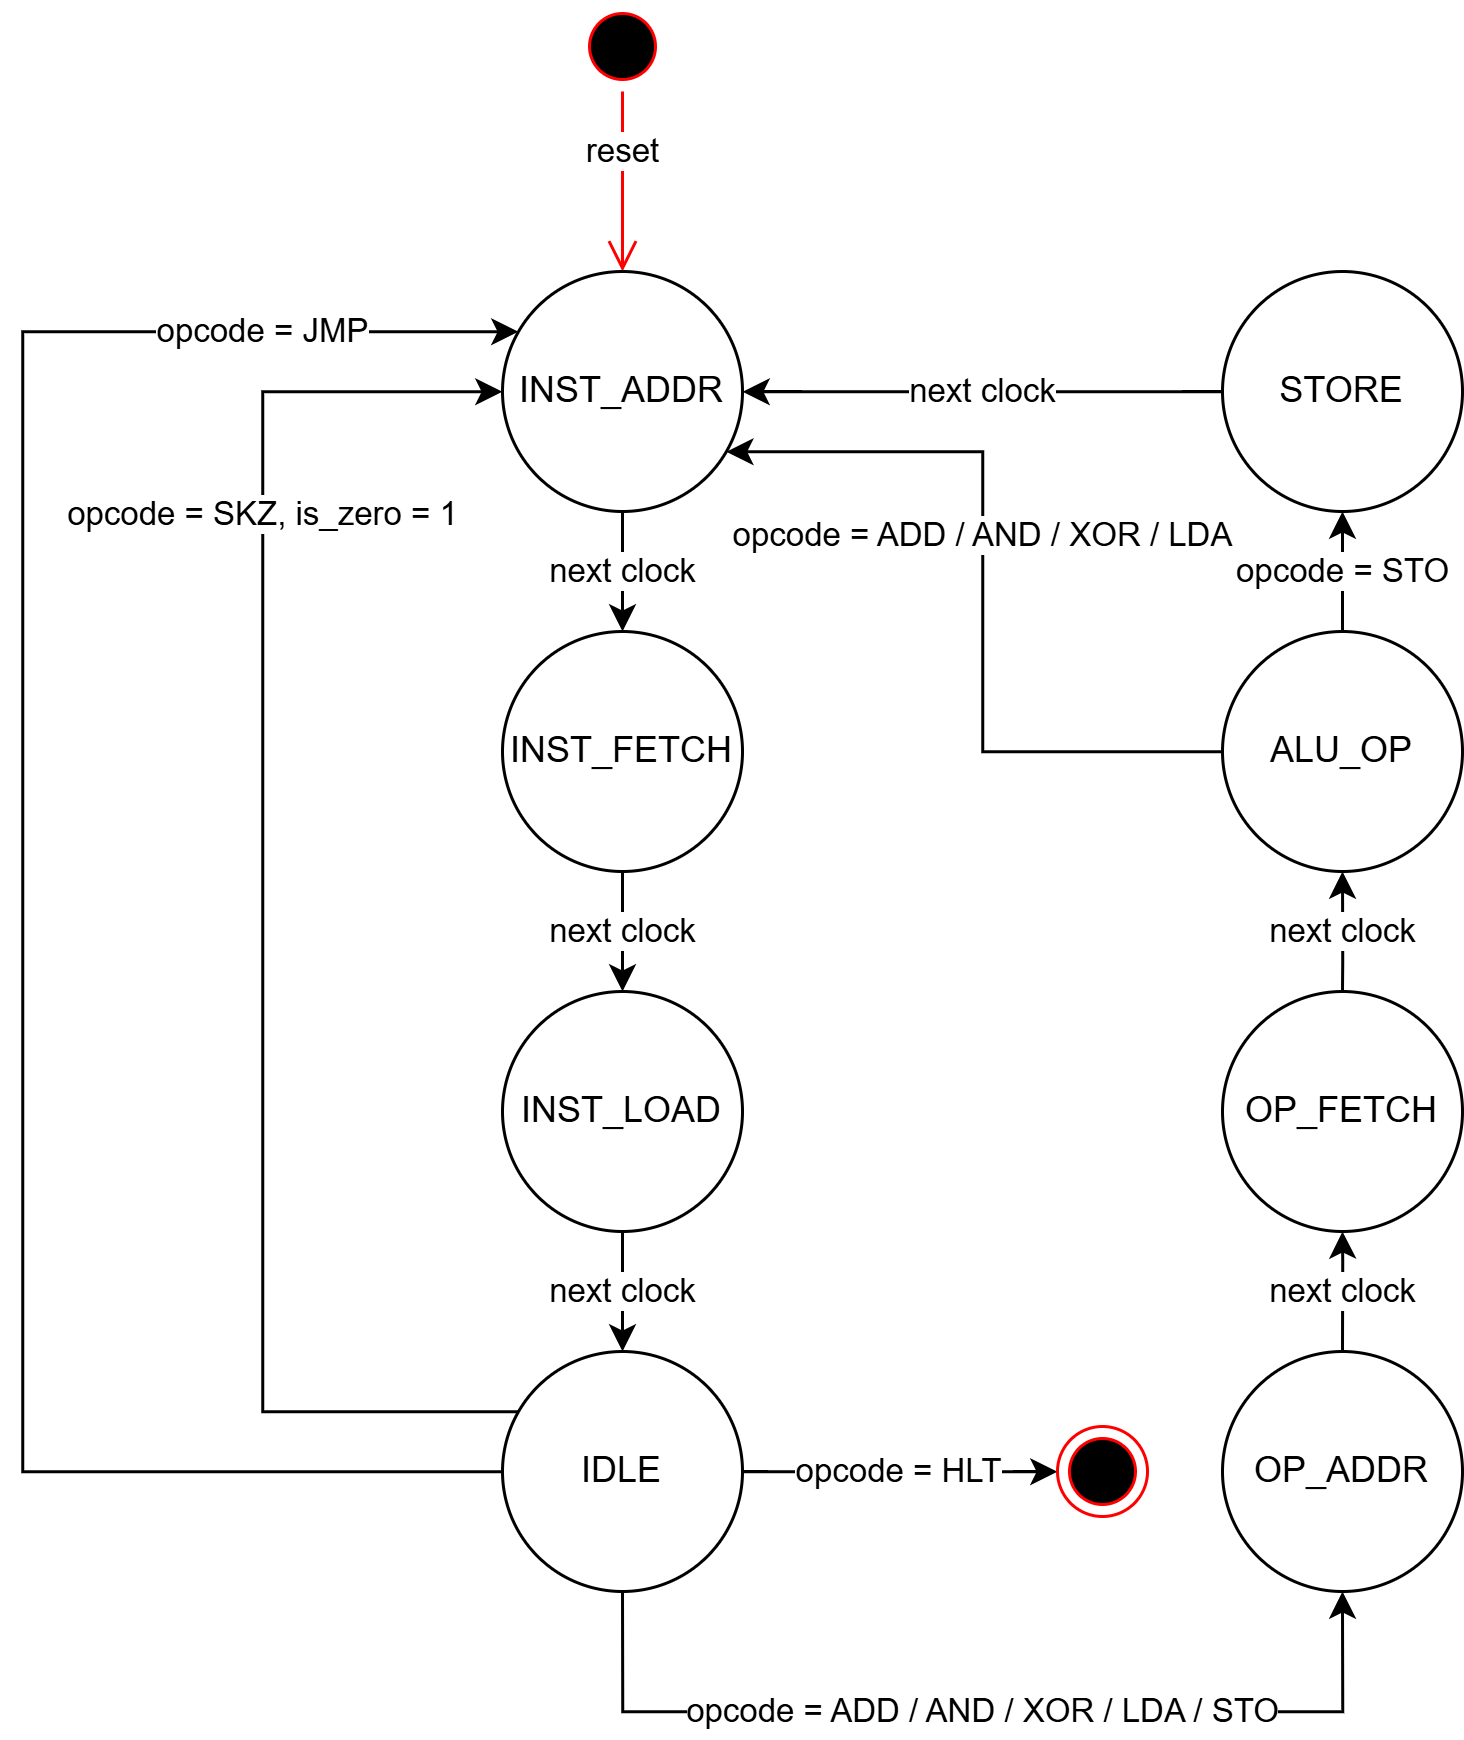
\includegraphics[width=0.8\textwidth]{graphics/RISC-CPU_FSM.drawio.png}
            \caption{Sơ đồ máy trạng thái của RISC-CPU}
        \end{figure}

        \begin{longtable}{|p{0.15\textwidth}|p{0.15\textwidth}|p{0.15\textwidth}|p{0.4\textwidth}|}
            \hline
            \textbf{Trạng thái} & \textbf{Điều kiện chuyển trạng thái} & \textbf{Trạng thái kế tiếp} & \textbf{Chức năng trạng thái} \\
            \hline
            \endfirsthead

            \hline
            \textbf{Trạng thái} & \textbf{Điều kiện chuyển trạng thái} & \textbf{Trạng thái kế tiếp} & \textbf{Chức năng trạng thái} \\
            \hline
            \endhead

            \hline
            \endfoot

            \hline
            \caption{Mô tả máy trạng thái của RISC-CPU}
            \endlastfoot

            \texttt{RESET} & Khi có tín hiệu \texttt{reset = 1} & \texttt{INST\_ADDR} & Đặt lại CPU, khởi động từ đầu chương trình. \\
            \hline
            \texttt{INST\_ADDR} & Sau 1 chu kỳ xung (\texttt{next clock}) & \texttt{INST\_FETCH} & Cung cấp địa chỉ lệnh từ PC để truy xuất lệnh từ bộ nhớ. \\
            \hline
            \texttt{INST\_FETCH} & \texttt{next clock} & \texttt{INST\_LOAD} & Đọc nội dung lệnh từ bộ nhớ. \\
            \hline
            \texttt{INST\_LOAD} & \texttt{next clock} & \texttt{IDLE} & Nạp nội dung lệnh vào Instruction Register. \\
            \hline
            \texttt{IDLE} & \texttt{opcode = HLT} & Dừng CPU & Kết thúc chương trình. \\
            \cline{2-4}
            & \texttt{opcode = SKZ} và \texttt{is\_zero = 1} & \texttt{INST\_ADDR} & Bỏ qua lệnh tiếp theo bằng cách tăng PC thêm 1 lần nữa. \\
            \cline{2-4}
            & \texttt{opcode = JMP} & \texttt{INST\_ADDR} & Nạp địa chỉ nhảy vào PC và tiếp tục thực thi từ địa chỉ mới. \\
            \cline{2-4}
            & \texttt{opcode = ADD / AND / XOR / LDA / STO} & \texttt{OP\_ADDR} & Bắt đầu xử lý các lệnh thao tác với bộ nhớ hoặc phép toán. \\
            \hline
            \texttt{OP\_ADDR} & \texttt{next clock} & \texttt{OP\_FETCH} & Cung cấp địa chỉ operand để truy xuất dữ liệu từ bộ nhớ. \\
            \hline
            \texttt{OP\_FETCH} & \texttt{next clock} & \texttt{ALU\_OP} & Đọc dữ liệu operand từ bộ nhớ. \\
            \hline
            \texttt{ALU\_OP} & \texttt{opcode = STO} & \texttt{STORE} & Ghi dữ liệu từ Accumulator xuống bộ nhớ. \\
            \cline{2-4}
            & \texttt{opcode = ADD / AND / XOR / LDA} & \texttt{INST\_ADDR} & Lưu kết quả phép toán vào Accumulator và quay lại vòng lặp lệnh. \\
            \hline
            \texttt{STORE} & \texttt{next clock} & \texttt{INST\_ADDR} & Ghi dữ liệu xuống bộ nhớ, sau đó trở về nạp lệnh mới. \\
            \hline
        \end{longtable}
\chapter{Simulation}
    \lstinputlisting[caption={Tên file Verilog}]{code/sample_verilog.v}

\input{contents/synthesis.tex}
\input{contents/lec.tex}



% \bibliographystyle{plain}
% \bibliography{refs/example.bib}
\nocite{*}

\end{document}
